\documentclass[11pt]{article}

\usepackage[english]{babel}
\usepackage[T1]{fontenc}
\usepackage[utf8x]{inputenc}

\usepackage{appendix}
\usepackage{amsmath}
\usepackage{cprotect}
\usepackage{listings}
\usepackage{float}
\usepackage[margin=2cm]{geometry}
\usepackage{graphicx}
\usepackage{underscore}
\usepackage{subcaption}

\graphicspath{ {assets/exer001/} }

\lstset{
    tabsize=3,
    breakatwhitespace=true,
    breaklines=true,
    frame=simple
}

\title{Exercise 1 - FPGA Simulated Annealing with VPR}
\author{Matthew Walker - 999540475 - walker82}
\date{\today}

% Placement
%   DONETODO score vs. temp (for each circuit)
%   TODO mean and stddev for at least 5 seeds
%   TODO add bump-up capability, repeat previous
%   TODO 5 temps X 5+ seeds, be sure to impact solution

% Routing
%   TODO run routing with W set, report post-routing crit. path delay
%   vary params to improve fmax
%   change pin-within-net and net ordering, report fmax

\begin{document}

\maketitle

\section{Simulated Annealing Placement}
\subsection{Baseline HPWL Placer}
\subsubsection{Cost vs Time/Temperature Plots}
\begin{figure}[ht]
\subcaptionbox{bigkey}{
	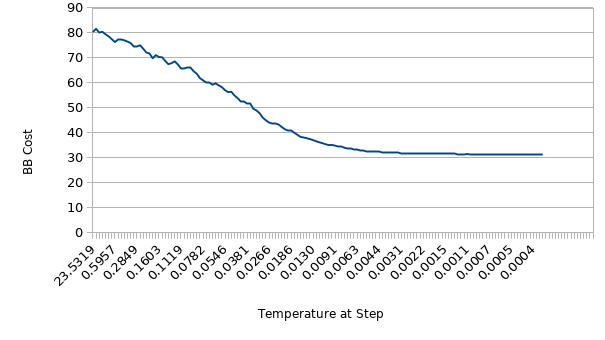
\includegraphics[width=0.5\linewidth]{bigkey-cost-at-step}}
\subcaptionbox{mkSMAdapter4B}{
	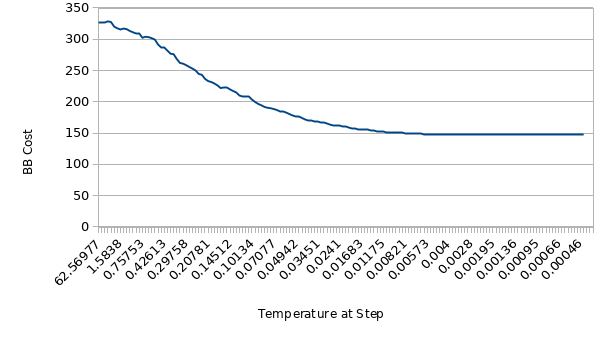
\includegraphics[width=0.5\linewidth]{mk-cost-at-step}}
\subcaptionbox{or1200}{
	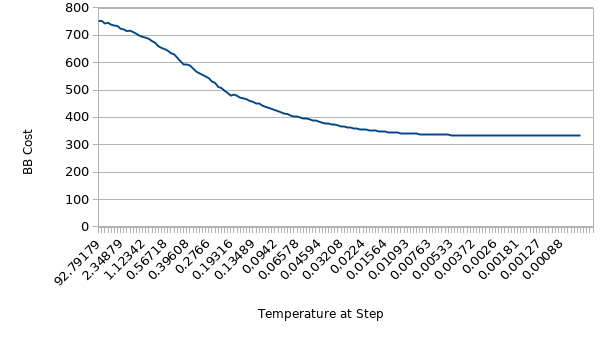
\includegraphics[width=0.5\linewidth]{or1200-cost-at-step}}
\subcaptionbox{pair}{
	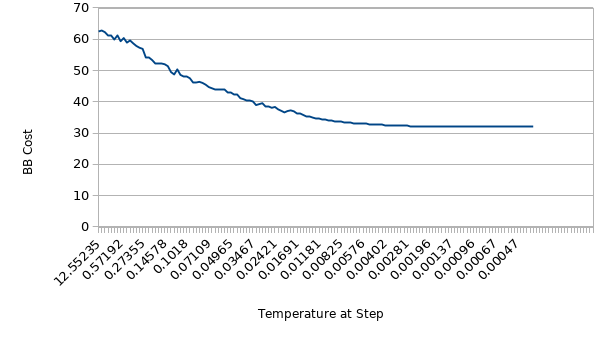
\includegraphics[width=0.5\linewidth]{pair-cost-at-step}}
\caption{HPWL cost over the course of placement (x \(\propto\) step number), with temperature labels.}
\label{fig:baseline-hpwl}
\end{figure}

\subsubsection{Seed Effects}

\begin{table} \centering
\begin{tabular}{l | *4r}
\hline\hline
circuit\textbackslash statistic & total blocks & total nets & total inputs & total outputs \\
\hline
bigkey & 1333 & 1136 & 229 & 197 \\
mkSMAdapter4B & 3513 & 3308 & 195 & 205 \\
or1200 & 4589 & 4258 & 385 & 394 \\
pair   & 791  &  654 & 173 & 137 \\
\hline\hline
\end{tabular}
\caption{Circuit statistics, after removing unused inputs.}
\label{tab:circuit-stats}
\end{table}

\begin{table}
\centering
\begin{tabular}{l | *{15}r}
\hline\hline
circuit\textbackslash init temp & 0.015 & 0.03 & 0.05 & 0.1 & 0.5 & 1 & 5 & 20 & 50 & 100 (default)\\
\hline
bigkey & 0.98 & 1.43 & 1.39 & 0.56 & 0.54 & 0.91 & 0.75 & 1.01 & 1.09 & 1.13 \\
mkSMAdapter4B & 4.73 & 3.96 & 5.25 & 3.62 & 1.93 & 2.65 & 1.97 & 2.21 & 1.59 & 1.90 \\
or1200 & 7.88 & 8.80 & 5.83 & 9.42 & 5.45 & 4.54 & 5.57 & 3.75 & 4.96 & 4.90 \\
pair & 1.22 & 0.76 & 0.76 & 0.45 & 0.62 & 0.62 & 0.39 & 0.52 & 0.37 & 0.45 \\
\hline\hline
\end{tabular}
\caption{Standard deviation of the final cost of 10 seeds of each circuit with various initial temperature settings. Default temperature adjustment schedule. }
\label{tab:stddev-by-temp}
\end{table}

\begin{table}
\centering
\begin{tabular}{l | *{15}r}
\hline\hline
circuit\textbackslash init temp & 0.015 & 0.03 & 0.05 & 0.1 & 0.5 & 1 & 5 & 20 & 50 & 100 (default)\\
\hline
bigkey & 2.3 & 3.6 & 3.8 & 1.6 & 1.4 & 2.4 & 2.0 & 2.7 & 2.9 & 3.0 \\
mkSMAdapter4B & 2.4 & 2.2 & 3.1 & 2.2 & 1.2 & 1.7 & 1.2 & 1.4 & 1.0 & 1.2 \\
or1200 & 1.8 & 2.2 & 1.5 & 2.5 & 1.5 & 1.3 & 1.6 & 1.0 & 1.4 & 1.4 \\
pair & 3.2 & 2.1 & 2.2 & 1.3 & 1.8 & 1.8 & 1.2 & 1.5 & 1.1 & 1.3 \\
\hline\hline
\end{tabular}
\caption{Standard deviation of the final cost of 10 seeds of each circuit with various initial temperature settings, as a percentage of the mean. Default temperature adjustment schedule. }
\label{tab:stddev-by-temp-as-percent}
\end{table}

\begin{table}
\centering
\begin{tabular}{l | *{15}r}
\hline\hline
circuit\textbackslash init temp & 0.015 & 0.03 & 0.05 & 0.1 & 0.5 & 1 & 5 & 20 & 50 & 100 (default)\\
\hline
bigkey & 42.7 & 39.2 & 37.0 & 36.2 & 37.8 & 37.9 & 38.1 & 37.5 & 37.1 & 37.6 \\
mkSMAdapter4B & 194.8 & 176.7 & 169.6 & 164.9 & 158.9 & 159.8 & 158.7 & 159.0 & 160.6 & 157.7 \\
or1200 & 438.7 & 401.4 & 383.9 & 375.2 & 359.4 & 359.8 & 359.4 & 359.0 & 358.5 & 356.7 \\
pair & 38.4 & 35.9 & 34.5 & 34.1 & 34.1 & 33.9 & 33.7 & 33.7 & 33.7 & 33.9 \\
\hline\hline
\end{tabular}
\caption{Mean final cost of 10 seeds of each circuit with various initial temperature settings. Default temperature adjustment schedule. }
\label{tab:mean-by-temp}
\end{table}

The circuits are similarly affected by noise when the standard deviation across seeds is normalized as a fraction of the mean (table \ref{tab:stddev-by-temp-as-percent}). However, when considered in absolute terms, the largest circuit, \emph{or1200} (see table \ref{tab:circuit-stats}), has the largest variation. Also, \emph{or1200}'s final cost is considerably higher than the only-slightly-smaller circuit \emph{mkSMAdapter4B}, suggesting that it has a significantly more difficult placement problem. Finally, there seems to be some dependency on circuit, as \emph{bigkey} has a somewhat larger variance, but middling statistics offering no explanation.

\end{document}
